\chapter{Preliminary Project Report}
\label{introduction}
\thispagestyle{plain}
\section{Introduction}
Every year, universities around the world, at the beginning of each term face the problem of creating a schedule or timetable for the subjects lectured. These timetables must satisfy the needs of a university and at the same time, attempt to satisfy as many of the wishes and requirements of both the university staff and students. The elaboration of these timetables done manually by administrative staff of the university is a time-consuming task which is both difficult and error prone. \\
Historically the timetabling problem has been considered a subject of the field of operational research, but in the last decades, it has also become a subject of research in the field of Artificial Intelligence, more specifically the application of \emph{metaheuristic} algorithms to solve these type of NP-hard problems ~\cite{Cooper1996, Even1976} (e.g. \emph{constraint satisfaction}, \emph{tabu search} and \emph{genetic algorithms} are examples of the techniques employed). \\
There is a lot of literature published regarding proposed solutions that are effective at solving these problems. After reading through some of these proposals, we infer that the formulation of the problem to solve is different in each proposal and usually adjusted to the rules and specific requirements of a given institution and the results obtained in the implementations of these solutions reflect this tight coupling. \\
The International Timetabling Competition (ITC)~\cite{McCollum} was established to stimulate interest in the general area of educational timetabling while providing researchers with models of the problems faced which incorporate an increased number of real world constraints.\\
This competition was divided in three tracks:
\begin{itemize}
\item[-] Track 1 - Examination Timetabling;
\item[-] Track 2 - Post Enrollment Based Course; Timetabling (PE-CTT)
\item[-] Track 3 - Curriculum Based Course Timetabling (CB-CTT).
\end{itemize}
For each track, it was provided the common generic formulation of the problem to solve, which in this case is the creation of feasible timetables and the hard and soft constraints that a proposed solution method must observe. In order to compare the results obtained with the proposed solution solvers, common datasets, representing real-word instances that represent the problem to solve, were provided. These order to give researchers a common set of benchmarks.\\
%%%%%%%%%%%%%%%
The goal of this project is to implement a solver program for the problem of Curriculum Based Course Timetabling as it was formulated in the Track 3~\cite{McCollum2010} of the second ITC competition that took place in 2007.\\
For this solver program, we propose the implementation of a Hybrid system, in which in the first stage a genetic algorithm (GA) is used to obtain a set of feasible solutions. In the second stage, the results obtained are processed by a local search algorithm – i.e. simulated annealing (SA) – in an attempt to further improve the quality of the solutions.\\
%%%%%%%%%%%%%%%
The resulting implementation will be tested with the ITC 2007 datasets, which in the case of track 3 corresponds to real datasets that were obtained from the university of Udine in Italy, and under some of the rules proposed in this competition. The results obtained will be compared both between the implemented solver and the results of the solutions proposed by the winner of the ITC 2007 Track 3~\cite{Mueller2007} in order to evaluate if the implemented solver can provide both better quality solutions and/or can be faster at obtaining these solutions.\\
%%%%%%%%%%%%%%%
\subsubsection{Document Organization}
This document is divided in the following sections:
\begin{enumerate}
\setcounter{enumi}{1}
\item Curriculum-Based Course Timetabling Problem - which presents the problem of the Curriculum-Based Course Timetabling.
\item State of the Art - an overview of several proposed approaches that deal with the timetabling problem.
\item Proposed solution - the selected algorithms that will later be implemented. We propose a hybrid solution that employs a GA to obtain a set of feasible solutions that will be further improved through the usage of local search algorithms, more specifically the SA algorithm.
\item Project Development Planning - the overall project plan.
\item Future Work - some topics that should be considered in the future.
\end{enumerate}
\section{Curriculum-Based Course Timetabling problem}
\label{cbcttproblem}
\thispagestyle{plain}
In this section, we present the formulation of the CB-CTT problem.
The specific problem of Curriculum-Based Course Timetabling, as proposed by Schaerf ~\cite{McCollum}, is an optimization problem which consists of the weekly scheduling of the lectures for several university courses within a given number of rooms and time periods. The conflicts between courses are set according to the curricula published by the University and not on the basis of enrolment data.\\
The problem consists of the following entities:
\begin{itemize}
\item[-] Days, Timeslots, and Periods - Given a number of teaching days in the week (typically 5 or 6) and considering that each day is split in a fixed number of timeslots, which are equal for all days. A period is considered to be a pair composed by a day and a timeslot. The total number of scheduling periods is the product of the days times the day timeslots. 
\item[-] Courses and Teachers - Each course consists of a fixed number of lectures to be scheduled in distinct periods, is attended by a given number of students, and is taught by a teacher. For each course there is a minimum number of days that the lectures of the course should be spread in, moreover there are some periods in which the course cannot be scheduled.
\item[-] Rooms - Each room has a capacity, which corresponds to the number of available seats. All rooms are equally suitable for all courses.
\item[-] Curricula - A curriculum is a group of courses such that any pair of courses in the group has students in common. Based on the curricula, we have conflicts between courses and other soft constraints. 
\end{itemize}
A feasible solution of the problem will correspond to an assignment of a period (day and timeslot) and a room to all lectures of each course and must conform to the following hard constraints:
\begin{itemize}
\item[-] Lectures - All lectures of a course must be scheduled and they must be assigned to distinct periods. 
\item[-] Room Occupancy - Two lectures cannot take place in the same room and in the same period. 
\item[-] Conflicts Lectures - of courses in the same curriculum or taught by the same teacher must be all scheduled in different periods.
\item[-] Availabilities - If the teacher of the course is not available to teach that course at a given period, then no lectures of the course can be scheduled at that period.
\end{itemize}
Additionally, the following soft constraints should be met as much as possible:
\begin{itemize}
\item[-] Room Capacity - For each lecture, the number of students that attend the course must be less or equal than the number of seats of all the rooms that host its lectures. 
\item[-] Minimum Working Days - The lectures of each course must be spread into a minimum number of days. 
\item[-] Curriculum Compactness Lectures belonging to a curriculum should be adjacent to each other (i.e., in consecutive periods). For a given curriculum we account for a violation every time there is one lecture not adjacent to any other lecture within the same day. 
\item[-] Room Stability - All lectures of a course should be given in the same room. 
\end{itemize}
A solution that conforms to these soft constraints is one that exhibits desired properties - e.g. coherent daily time slots for lectures of the same curriculum.
\section{State of the Art}
In this section, we brifly describe some approaches devised to solve the problem automated construction of timetables. This is a research field for which extensive literature exists. Carter~\cite{Carter1986} proposed a categorization of four types of methods that can be used to solve this type of problem: sequential methods, cluster methods, constraint-based methods and generalized search. Petrovic et al.~\cite{Petrovic2004} proposed additional methods, such as hybrid evolutionary algorithms, meta-heuristics, multi-criteria approaches, hyper-heuristics and adaptive approaches.\\
Socha et al.~\cite{Socha2002} proposed an approach to tackle the course timetabling problem that applied local search and ant colony optimization strategies. Rossi-Doria et al.~\cite{Rossi-Doria2003} proposed the usage of evolutionary algorithms to solve the timetabling problem and presented a comparison between this method and several metaheuristic methods.
Burke et al.~\cite{Burke2003} applied a tabu-based hyper-heuristic to the university course timetabling problem. Burke et al.~\cite{Burke2007} proposed the use of tabu search along with a graph based hyper-heuristic. Abdullah et al.~\cite{Abdullah2005} developed a variable neighborhood search approach in conjunction with a tabu list. McMullan~\cite{McMullan2007} proposed the application of an extended great deluge algorithm and Landa-Silva et al.~\cite{Landa-Silva2008} presented another variation of the great deluge algorithm, the non-linear great deluge. The combination of genetic algorithm and local search has been employed by Abdullah et al.~\cite{Abdullah2008}.\\
Müller~\cite{Mueller2007} presented a constraint-based solver to the curriculum-based course timetabling problems in the 2nd International Timetabling Competition, ITC 2007 (Track 1 and Track 3) and achieved the first place in this competition. Lü et al.~\cite{Lue2010} applied a hybrid heuristic algorithm called Adaptive Tabu Search (ATS) to the same instances. Clark et al.~\cite{Clark2008} applied repair-based heuristic search on Track 3 datasets in the ITC 2007 timetabling competition. Geiger~\cite{Geiger2008} applied a stochastic neighborhood method based on threshold acceptance criteria to overcome the local optima to the same instances. Atsuta et al.~\cite{Atsuta2007} applied the constraint satisfaction problem (CSP) which implemented a hybridization of tabu search and iterated local search algorithms to handle weighted constraints.\\
De Cesco et al.~\cite{DeCesco2008} applied a dynamic tabu search to curriculum-based course timetabling, a short term tabu exclusion with variable size tabu length, with dynamic weight adjustment for hard and soft constraints.\\
Lach et al.~\cite{Lach2008} applied an integer programming method in order to create a solver to handle timetabling problem instances.\\
Burke et al.~\cite{Burke2009} proposed a solver based on a hybrid meta-heuristic to tackle scheduling problems.\\
Surveys that document these and additional approaches that handle these type of problems, can be consulted in several works such as Carter et al.~\cite{Carter1996}, Burke et al.~\cite{Burke2002}, Carter~\cite{Carter1986}, and Schaerf~\cite{Schaerf1999}.
\section{Proposed Solution}
\label{implementation}
\subsubsection{Overview}
\label{subsubsec:solution-overview}
After researching through the various proposals for solving different timetabling problems (e.g. ~\cite{Bajeh2001},~\cite{Chiarandini2006}) it became clear that although genetic algorithms (GA) are an appropriate method to solve this type of problem, it also became clear that it’s usage is not efficient in terms of time and computation effort needed to attain feasible solutions, when compared with other strategies such as tabu search or simulated annealing. In fact, the work submitted by Chiarandini et al. ~\cite{Chiarandini2006} proposes that the usage of meta-heuristic algorithms such as GA and Ant Colony Optimization (ACO) alone should be hybridized with local search procedures in order to achieve good results.\\
With this in mind and since the ITC 2007 rules~\cite{McCollum2007} for evaluating the algorithms indicate that the solutions must be produced within a time limit, it became apparent that it would be more appropriate to explore a hybrid approach, in which:
\begin{itemize}
\item[-] A GA is used to create the initial feasible solutions 
\item[-]	A local search algorithm, i.e. Simulated Annealing, is applied over the results produced by the GA in order to improve the quality of solutions.
\end{itemize}
The general overview of this is depicted in Figure~\ref{fig:overviewProposedApproach}.\\
\vspace{0.2cm}
\begin{figure}[h!]
 \centering
   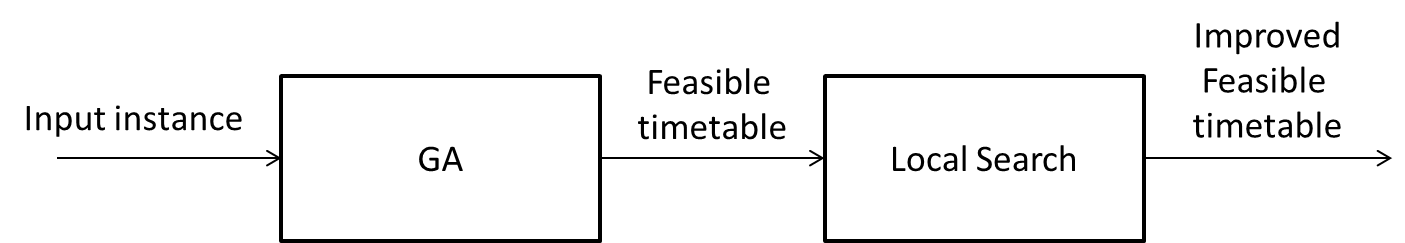
\includegraphics[width=10.5cm]{./images/figures/Fig1_OverviewProposedApproach.png}
   \caption{Overview of the proposed approach.}
   \label{fig:overviewProposedApproach}
\end{figure}\\
\subsubsection{First Phase - Genetic Algorithm}
\label{subsubsec:genetic-algorithm}
In the first stage, for the proposed genetic algorithm, only the hard constraints are considered, meaning that the fitness function used in this stage, will take into account only the violations of hard constraints, in an attempt to produce feasible timetables where all of these constraints are satisfied.\\
It’s expected that in the end of this first stage, the algorithm will have produced at least one feasible timetable and it will initiate the second stage if and only if a feasible timetable is found.\\ 
Figure~\ref{fig:overviewProposedSteps} ilustrates the steps that will be executed by the algorithm.\\
\begin{figure}[h!]
 \centering
   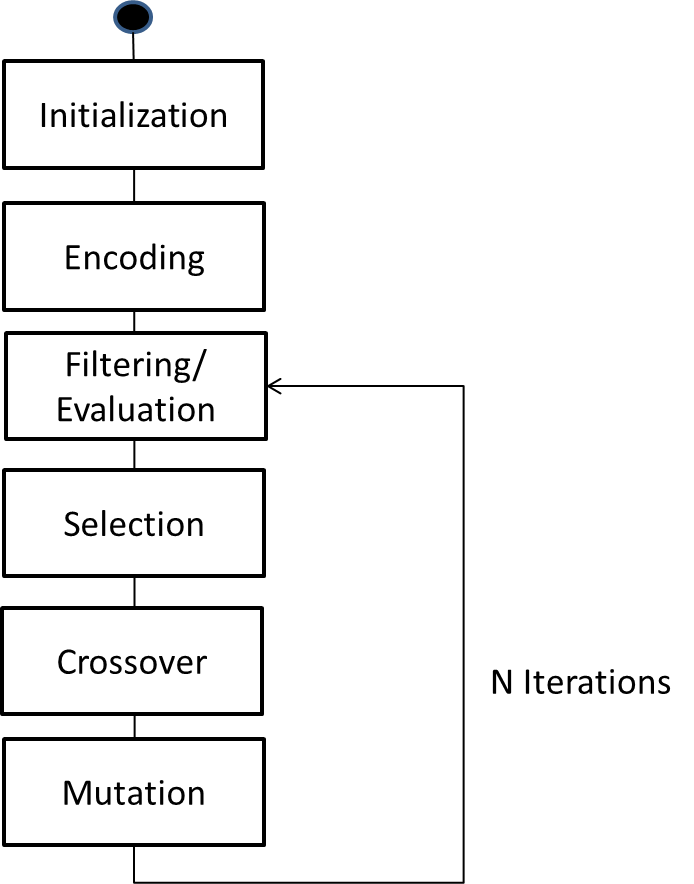
\includegraphics[width=12cm]{./images/figures/Fig2_OverviewSteps_GA.png}
   \caption{Overview of the steps of the proposed genetic algorithm.}
   \label{fig:overviewProposedSteps}
\end{figure}\\
The following subtopics present an overview of the implementation considerations that will be taken into account in each one of these steps.\\
\subsubsection{Initialization}
\label{subsubsubsec:ga-initialization}
The algorithm in the initialization step will create a set of initial solutions. In this stage we intend to use a sequential greedy heuristic as proposed by Lü et al. ~\cite{Lue2010} starting from an empty timetable, this heuristic constructs assignments by inserting one appropriate lecture into the timetable at each time. At each step, two distinct operations are carried out: one is to select a still unassigned lecture of a course and the other is to determine a period-room pair for this lecture.\\
The algorithm does not place a course lecture in a timeslot which is not available for that course, and will attempt to satisfy this constraint satisfied in the next generations for as long as possible.  After the completion of the generation of the population, the resulting timetables will be encoded as chromosomes.\\
\subsubsection{Encoding}
\label{subsubsubsec:ga-encoding}
The proposal for encoding the chromosomes that represent the timetables consists of using a 1-dimensional array of binary values, with a structure such as the one in Figure~\ref{fig:chromosomeRepresentation}.\\ 
\begin{figure}[h!]
 \centering
   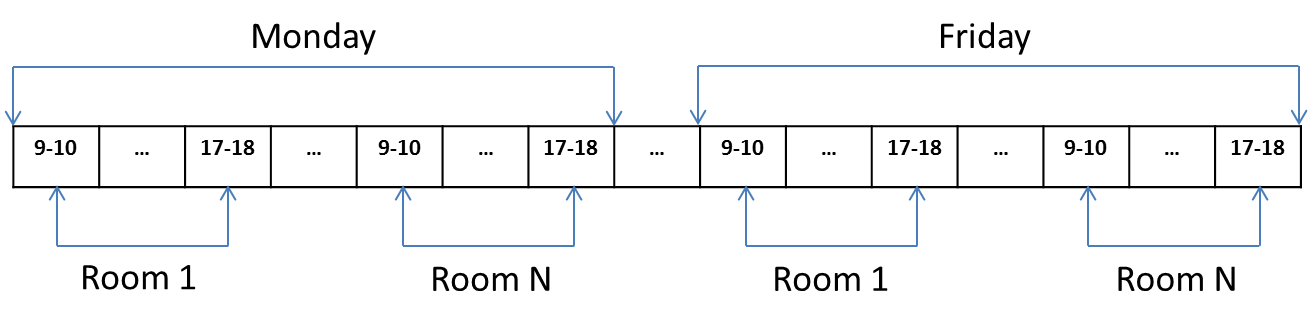
\includegraphics[width=12cm]{./images/figures/Fig3_ChromosomeRepresentation_GA.png}
   \caption{Chromosome representation.}
   \label{fig:chromosomeRepresentation}
\end{figure}\\
Each cell in the array represents a timeslot. A group of X adjacent timeslots represents one day of lectures that can be assigned in a single room. A group of Y adjacent room-timeslots represents the total number of lectures that can be allocated on that given day. Value 0 represents that the timeslot is available for allocation, 1 represents that it is already alocated.\\
The information regarding the lecturer, curriculum, etc. will be maintained on an associative array that will keep the information regarding the current allocated position in this array.\\
\subsubsection{Evaluation}
\label{subsubsubsec:ga-evaluation}
A fitness value is assigned to each timetable based on the number of violations of hard and soft constraints detected. In each generation the chromosomes are evaluated and then the chromosome pool is sorted. The evaluation process employs a fitness function to calculate the fitness of each timetable.\\
\subsubsection{Selection}
\label{subsubsubsec:ga-selection}
In the selection step, the fittest individual will be kept unchanged. The remaining individuals will subjected to a selection method in order to determine which indviduals are elected to perform the crossover and generate new individuals. A analysis between different selection methods - e.g. tournament selection, roulette selection, etc. - will be conducted during the implementation phase of the project, in order to evaluate which of the selection methods provide the best results.\\
\subsubsection{Crossover}
\label{subsubsubsec:ga-selection}
During the implementation phase, experiments with different types of crossover operators – e.g. One-Point Crossover, Two-Point Crossover, N-Points Crossover – will be conducted in order to evaluate which one of these is more adequate to generate the offspring.\\
\subsubsection{Mutation}
\label{subsubsubsec:ga-mutation}
The mutation function randomly exchanges the values in every pair in a random number of location pairs of a timetable. The mutation rate is not fixed. In each generation the maximum and average fitness values will be computed. If the two numbers are close enough to each other, the mutation rate value will be increased to avoid any chance of an early convergence.\\
\subsubsection{Repair Function}
\label{subsubsubsec:ga-repairfunction}
It is expected that the application of the crossover and mutation operators  will produce non feasible solutions, possibly with the worst fitness values than the least fit individuals that were determined in the selection step. Therefore, instead of purging the K least fit individuals immediately after the crossover step, a new fitness evaluation will be performed over the new population along with the least fit individuals that were not purged. After this evaluation step, the new K least fit individuals group will be purged, and a new iteration of the process will begin.
%%%%%%%%%%%%%%%
\subsubsection{Second Phase - Simulated Annealing Algorithm}
\label{subsubsec:genetic-algorithm}
Simulated annealing (SA) has been widely used to solve combinatorial optimization problems. It accepts the new solution when the objective value, which is determined by an objective function, is lower than or equals to the current one (considering a minimization problem). There is a probability to accept a worst quality solution using a probability acceptance function which controls the acceptance of the new solution. The current temperature is iteratively reduced according to the cooling schedule with a given cooling rate in each iteration or level until its temperature reaches the final minimum temperature, which is close to zero.\\ 
When the SA temperature becomes very low, the SA will exhibit a behavior similar to a descent heuristic (i.e, accepts only an improving solution) and therefore the search might be trapped in local optimum. To limit this effect, reheating will be used, in order to attempt to restart the search in another point in the search space.\\
The proposed SA algorithm will involve defining the neighborhood structure that should be considered and the cooling schedule strategy. 
The following items represent the termination criteria, used in the proposed SA:
\begin{itemize}
\item[-] The minimum temperature is close to zero 
\item[-] Number of iterations reaches the limit
\item[-] Timeout based on the ITC 2007 course timetabling track 3 stopping condition.
\end{itemize}
\subsubsection{General System Architecture Overview}
\label{subsubsec:solution-architecture-overview}
In this section we discuss the general system architecture that will be implemented. Figure~\ref{fig:systemArchitecture} illustrates the proposed architecture.\\
\begin{figure}[h!]
 \centering
   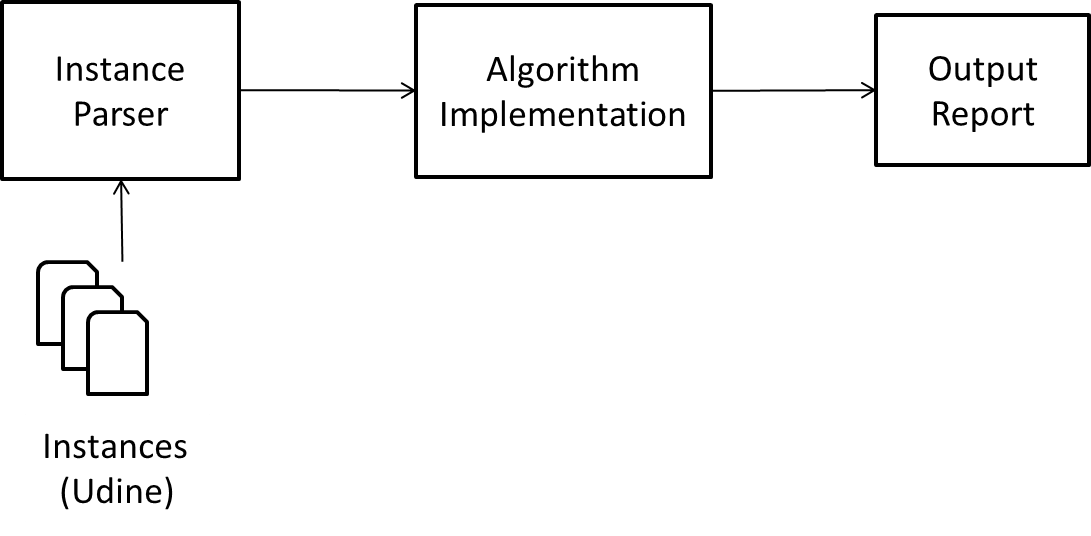
\includegraphics[width=12cm]{./images/figures/Fig4_SystemArchitecture.png}
   \caption{General System Architecture.}
   \label{fig:systemArchitecture}
\end{figure}\\
The instance parser is the component responsible for parsing the problem instances that were provided by the University of Udine for the ITC 2007 Track 3 competition. The instances will be loaded in memory. After the instances are loaded, the implemented algorithms modules will be executed. After the completion of the execution, a report file will be generated with the information regarding the best solution and data regarding metrics (e.g. Time executed, CPU time, etc).\\
The system will be implemented as a normal Java console application. The motivation regarding the usage of Java for the implementation is the availability of third party components that can be useful in the data manipulation and visualization, which can benefit the analysis of the results. \\
As a general requirement, the application should be able to obtain configuration data that can be used to perform the tuning of parameters used in the solver algorithms (e.g. the parameters used in the cooling schedule of the simulated annealing algorithm).
%%%%%%%%%%%%%%%
\section{Project Planning}
\label{planning}
\thispagestyle{plain}
This project is comprised by two phases. The first phase, which is currently completed, consisted on the research of the timetabling problem, with emphasis on the ITC 2007 Track 3 Curriculum-Based Timetable problem, and several meta-heuristic algorithms that are used to create automated solvers. In this phase, we also selected the algorithms that will be implemented and defined the way in which the obtained results with each implementation will be analyzed.\\
The graphic in Figure~\ref{fig:completedTasks} presents the allocation of time (expressed in terms of percentage) to the most relevant tasks that were executed in the first phase of this project.\\
\begin{figure}[h!]
 \centering
   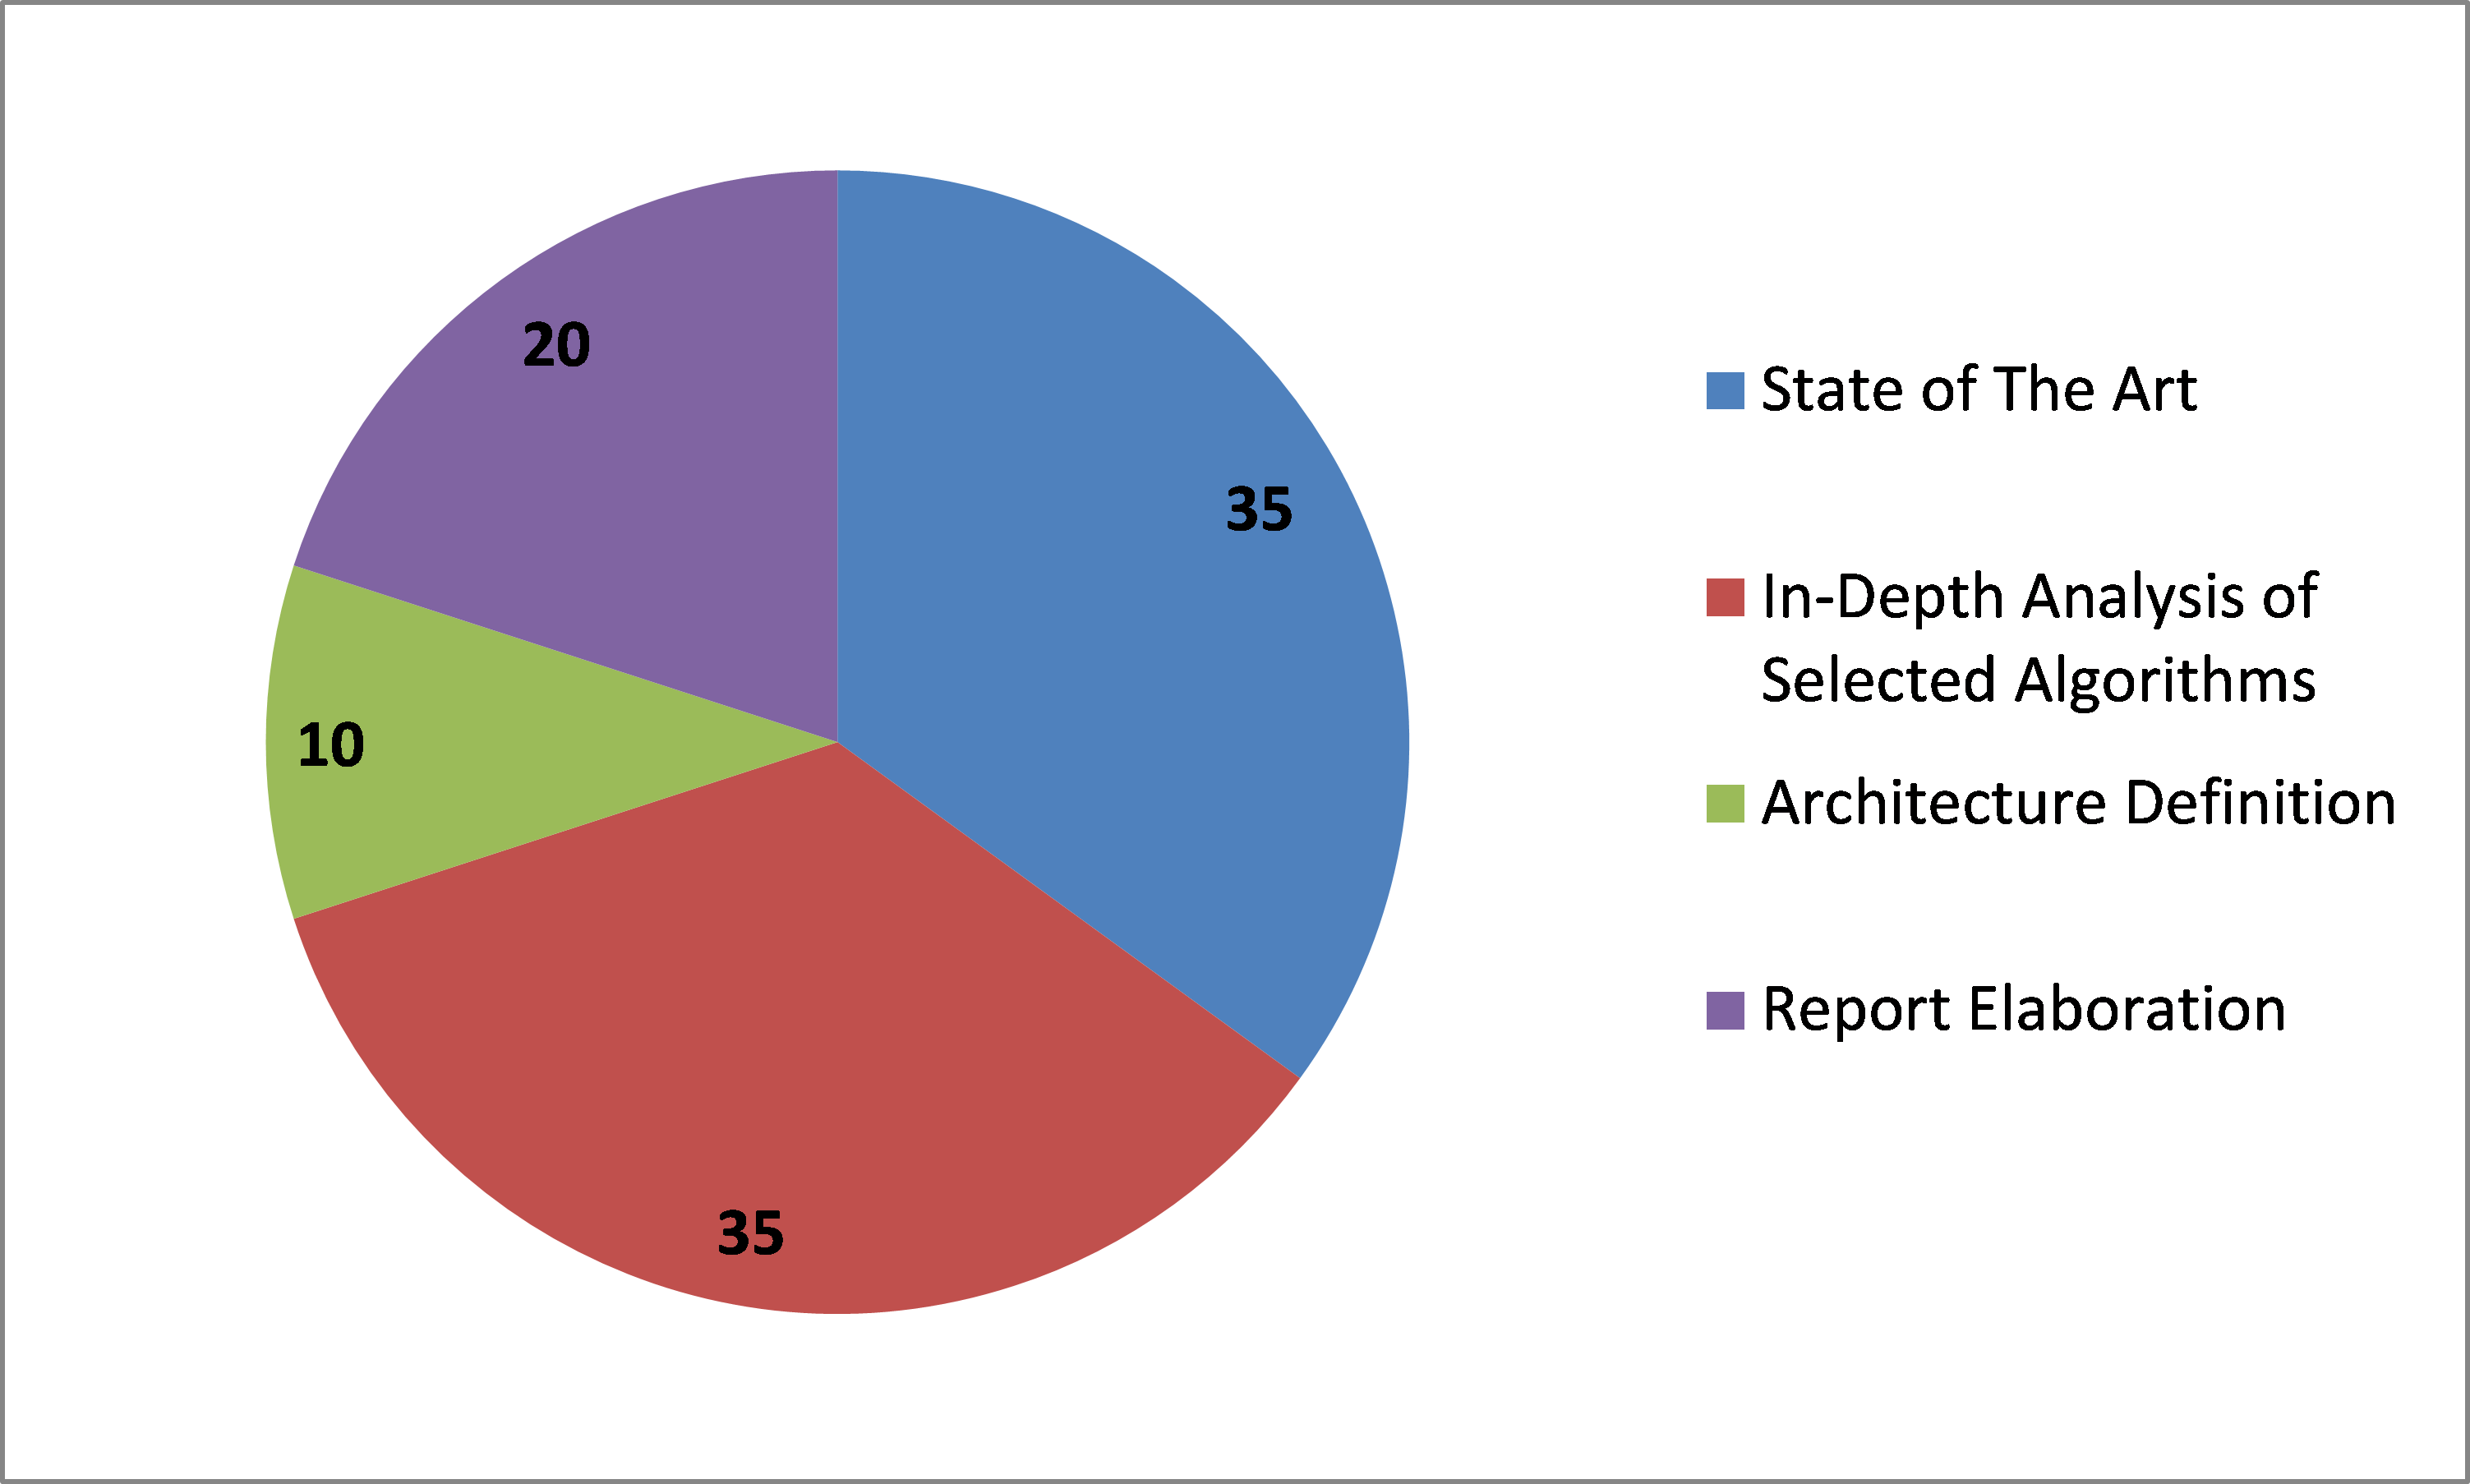
\includegraphics[width=6.36cm]{./images/figures/Fig5_CompletedProjectTasks.png}
   \caption{Allocation of time to the tasks executed in the first phase.}
   \label{fig:completedTasks}
\end{figure}\\
The GANT diagram depicted in Figure~\ref{fig:ganttDiagram} illustrates a detailed planning for the whole year. It includes all the relevant tasks related to the first and second phases of the project development. The second phase (and pending) tasks are represented in blue.\\
\begin{figure}[h!]
 \centering
   \hspace*{-2cm}
   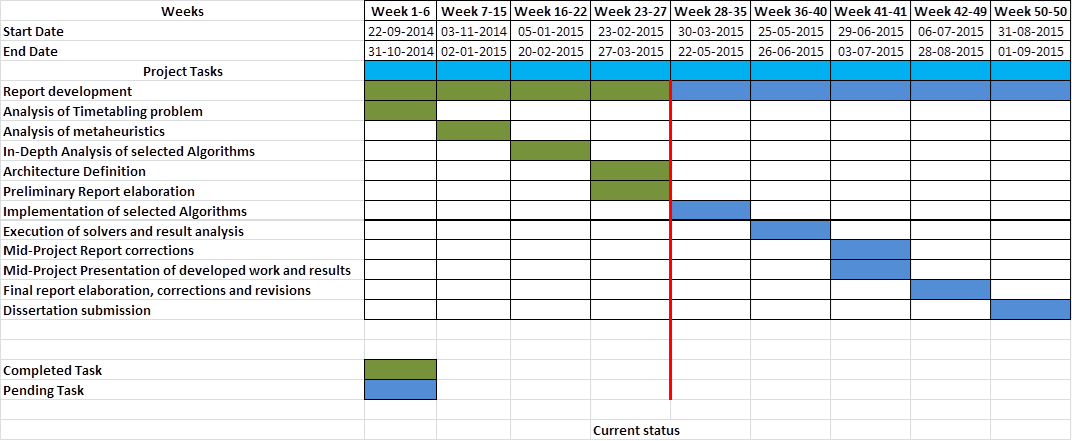
\includegraphics[width=20cm]{./images/figures/Fig6_GANTT_Diagram.png}
   \caption{GANTT diagram detailing the project plan.}
   \label{fig:ganttDiagram}
\end{figure}\\
Some changes to the proposed plan may occur during the project development, influencing the duration and final proposed dates for some tasks may. The time distribution and amount of work to be accomplished between the winter and summer periods is not equally distributed. This is because of the courses taken by the author during the winter semester in parallel with the project development, which consumed a lot of time of the winter period.\\
\section{Future Work}
\label{subsubsec:future-work}
In the following project phase, we will initiate the implementation of the algorithms. Upon completion of the implementation, we will initiate the execution of the algorithms over the provided instances and afterwards will analyze the results obtained and compare them with the ITC 2007 winning implementation results.\\
\let\cleardoublepage\clearpage